\documentclass[a4paper,12pt]{article}
\usepackage{dsfont}
\usepackage{amsmath,amssymb,amsthm,bm}
\usepackage{subfigure}
\usepackage{graphicx}
\usepackage{indentfirst}
\usepackage{url,booktabs}
\usepackage{multirow}
\usepackage{algpseudocode}
\usepackage{algorithm}
\usepackage{hyperref,xcolor}
\usepackage[portuguese]{babel}    	% para texto em Português
\usepackage{xcolor}	
\usepackage{listings}	
\usepackage[utf8]{inputenc}   % para acentuação em Português OU
\usepackage{epstopdf}



\begin{document}
Nome:Arthur Carneiro Leão Machado.
\vskip
Professor: Raydonal Ospina Martínez.
\vskip 
Disciplina: Estatística Não Paramétrica.

\section{Introdução}
O método de Monte Carlo, baseia-se em amostragens aleatórias massivas, repetindo sucessivas simulações a um elevado número de vezes, sendo assim, querendo medir com maior exatidão testes definidos no estudo.\\
\begin{equation}
    \pi(\theta) = 1- \beta
\end{equation}
Sendo $\beta$ a probabilidade de ocorrer o erro tipo 2.
O Poder do Teste tem como objetivo conhecer o quanto o teste de hipóteses controla um erro do tipo II, ou qual a probabilidade de rejeitar a hipótese nula se realmente for falsa.
O estudo será a respeito desse poder, utilizando uma estatística $t$, para testar a Hipótese: $H_0: \mu = 0.5$ \texit{\versus} $H_1: \mu  > 0.5 $, em que $\mu_0$ são as médias de cada população de interesse.
As populaçãoes geradas no Comando R, são: $Normal(0.5,1)$; $Exponencial(2)$; $Uniforme(0,1);$ $Cauchy(0.5,1)$; $ Log Normal(0.5,1)$. O estudo contará com o desempenho da função poder, quando aumentamos o tamanho da amostra, sendo analisado, quando $n=20, 40, 50, 100$, tudo isso a um nível de significância $\alpha = 5\%$. 

\section{Resultados}
 Podemos analisar na figura 1, sendo uma população normal que quando mais aumentamos o tamanho da amostra, como por exemplo, para $n=100$, maior é o poder do teste. A respeito de uma população com distribuição Uniforme, podemos analisar pela figura 2, que o poder do teste obteve uma caráter menos liberal, sendo ele mais consistente, independente do tamanho da amostra, sendo isso uma certa peculiaridade. No caso da distribuição Exponencial, apresenta-se o mesmo caso de uma população normal, o poder do teste sendo influenciado pelo tamanho da amostra. Na distribuição Log Normal, ela apresenta uma situação um pouco diferente quando fizermos o caso para $n=40$, apresentando uma grande mudança em relação ao caso com $n=20$, aumentando drasticamente poder do teste. Finalmente, o caso de uma população com distribuição cauchy, apresenta de fato, o menor poder entre todos analisados anteriormente, sendo aparente a sua não dependencia de $n$, essa peculiaridade pode ser explicada porque sua média é definida, mas não existe.



\begin{figure}[H]
	\centering
	\textbf{Figura 1} : Gráfico de Poder usando Método de Monte Carlo para uma população com Distribuição Normal.
	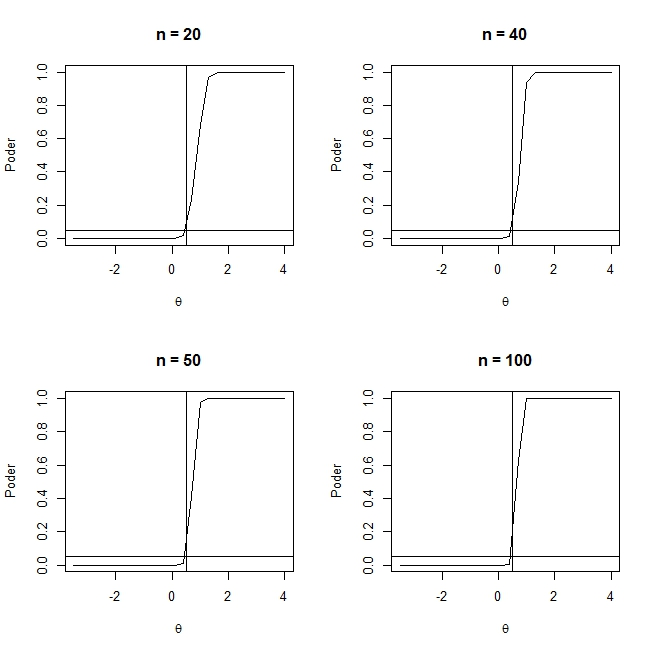
\includegraphics[width=0.60\textwidth]{Normal.jpeg}\\~\\
	\textbf{Figura 2} : Gráfico de Poder usando Método de Monte Carlo para uma população com Distribuição Uniforme.
	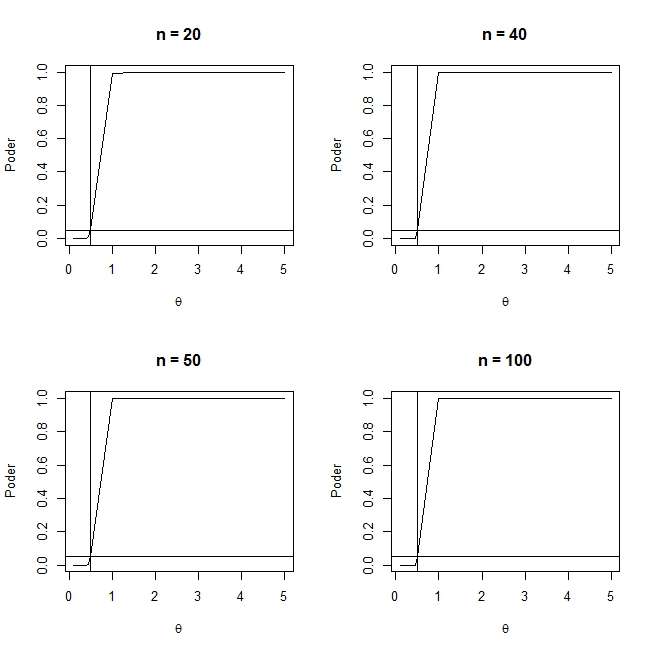
\includegraphics[width=0.60\textwidth]{Uniforme.jpeg}\\~\\
	\label{Rotulo}
\end{figure}


\begin{figure}[H]
	\centering
	\textbf{Figura 3} : Gráfico de Poder usando Método de Monte Carlo para uma população com Distribuição Exponencial.
	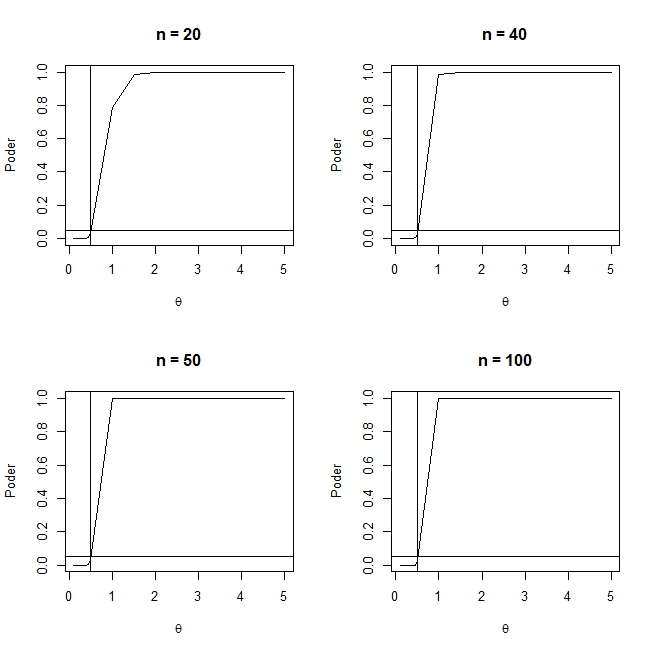
\includegraphics[width=0.60\textwidth]{Exponencial.jpeg}\\~\\
	\textbf{Figura 4} : Gráfico de Poder usando Método de Monte Carlo para uma população com Distribuição Log Normal
	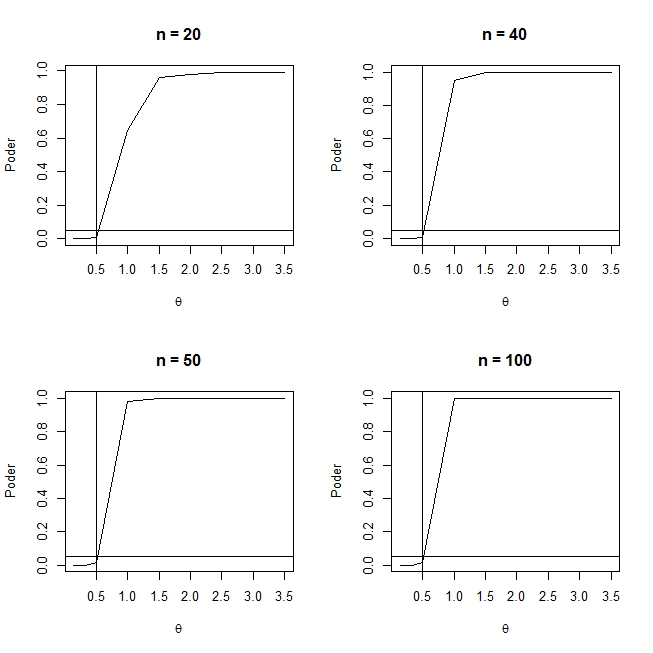
\includegraphics[width=0.60\textwidth]{LogNormal.jpeg}
	\label{Rotulo}
\end{figure}

\begin{figure}[H]
	\centering
	\textbf{Figura 5} : Gráfico de Poder usando Método de Monte Carlo para uma população com Distribuição Cauchy.
	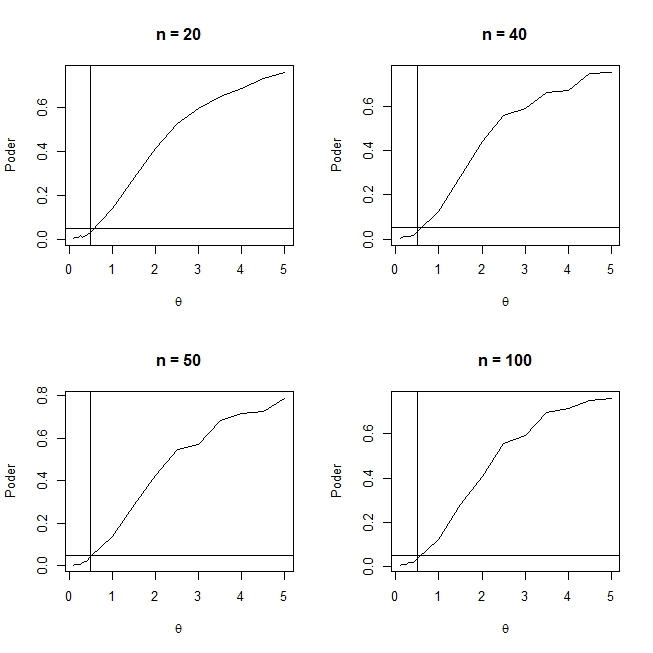
\includegraphics[width=0.60\textwidth]{Cauchy.jpeg}
	\label{Rotulo}
\end{figure}

\end{document}
